\chapter{\label{ch_lcm}The LCM Contention Manager}
\markright{Mohammed El-Shambakey \hfill Chapter~\ref{ch_lcm}. LCM \hfill}
%
\textbf{RE-READ THIS INTRODUCTION AFTER FINISHING CHAPTER}
Under ECM and RCM, each atomic section can be aborted for at most $2.s_{max}$ by a single interfering atomic section. We present a novel contention manager (CM) for resolving transactional conflicts, called length-based CM (or LCM)~\cite{lcmdac2012}. LCM can reduce the abortion time of a single atomic section due to an interfering atomic section below $2.s_{max}$. We upper bound transactional retries and response times under LCM, when used with G-EDF and  G-RMA schedulers. We identify the conditions under which LCM outperforms previous real-time STM CMs and lock-free synchronization.
\begin{comment}
 Our implementation and experimental studies reveal that G-EDF/LCM and G-RMA/LCM have shorter or comparable retry costs and response times than other synchronization techniques.
\end{comment}

The rest of this Chapter is organized as follows: Section~\ref{sec:lcm} presents Length-based Contention Manager (LCM) and illustrates its behaviour. Section~\ref{sec:lcm_properties} derives LCM properties. Response time analysis of tasks under G-EDF/LCM is given in Section~\ref{response g-edf/lcm}. Schedulability of G-EDF/LCM is compared to schedulability of ECM and lock-free in Section~\ref{performance g-edf-lcm}. Section~\ref{rma} gives response time analysis for G-RMA/LCM. Schedulability of G-RMA/LCM is compared against RCM and lock-free in Section~\ref{rma eval}. We conclude Chapter in Section~\ref{sec:conclusions_lcm}.
%
\section{\label{sec:lcm}Length-based CM}
%
LCM resolves conflicts based on the priority of conflicting transactions, besides the length of the interfering atomic section, and the length of the interfered atomic section. Priority of each transaction equals priority of its containing job (i.e., $p\left(s_i^k\right)=p_i^x$ where $s_i^k \in \tau_i^x$). ECM and RCM (Chapter~\ref{ecm-rcm}) use only priorities to resolve conflicts. LCM allows lower priority jobs to retry for lesser time than that under ECM and RCM, but higher priority jobs, sometimes, wait for lower priority ones with bounded priority-inversion.

\subsection{\label{sec 9.1}Design and Rationale}
%
\begin{algorithm}
\footnotesize{
\LinesNumbered
\KwData{$s_i^k$ and $s_j^l$ are two conflicting atomic sections.\\$\psi\rightarrow$ predefined threshold $\in [0,1]$.\\$\delta_i^k \rightarrow$ remaining execution length of $s_i^k$.\\
$s\left(s_i^k\right) \rightarrow$ start time of $s_i^k$. $s\left(s_i^k\right)$ is updated each time $s_i^k$ aborts and retries to the start time of the new retry.\\
$s\left(s_j^l\right) \rightarrow$ the same as $s\left(s_i^k\right)$ but for $s_j^l$.
}
\KwResult{which atomic section of $s_i^k$ or $s_j^l$ aborts}
\eIf{$s\left(s_i^k\right) < s\left(s_j^l\right)$\label{lcm:s_i_k start before s_j_l}}
{
\eIf{$p\left(s_i^k\right) > p\left(s_j^l\right)$}
	{$s_j^l$ aborts\label{lcm:step_sicommits}\;}
	{$c_{ij}^{kl}=len(s_j^l)/len(s_i^k)$\label{step_cijkl}\;
	$\alpha_{ij}^{kl}=ln(\psi)/(ln(\psi)-c_{ij}^{kl})$\label{step_alphaijkl}\;
	$\alpha=\left(len(s_i^k)-\delta_i^k\right)/len(s_i^k)$\label{step_alpha}\;
	\eIf{$\alpha \le \alpha_{ij}^{kl}$}
	{$s_i^k$ aborts\label{lcm:step_siaborts}\;}
	{$s_j^l$ aborts\label{step_sjaborts}\;}
	}
	}
	{
	Swap $s_i^k$ and $s_j^l$\label{lcm:s_j_l start before s_i_k}\;
	}
	}
\caption{LCM}
\label{alg_lcm}
\end{algorithm}
%
For both ECM and RCM, $s_{i}^{k}$ can be totally repeated if $s_{j}^{l}$ --- which belongs to a higher priority job $\tau_{j}^b$ than $\tau_{i}^a$ --- conflicts with $s_{i}^{k}$
at the end of its execution, while $s_{i}^{k}$ is just about
to commit. Thus, LCM, shown in Algorithm~\ref{alg_lcm}, uses the remaining length of $s_{i}^{k}$ when it is interfered,
as well as $len(s_{j}^{l})$, to decide which transaction must be aborted. If $s_i^k$ starts before $s_j^l$, then $s_i^k$ is the interfered atomic section and $s_j^l$ is the interfering atomic section (step~\ref{lcm:s_i_k start before s_j_l}). Otherwise, $s_i^k$ and $s_j^l$ are swapped (step~\ref{lcm:s_j_l start before s_i_k}). If $p\left(s_i^k\right)$ was greater than $p\left(s_j^l\right)$, then $s_i^k$ would be the one that commits, because it belongs to a higher priority job, and it started before $s_j^l$ (step~\ref{lcm:step_sicommits}). Otherwise, $c_{ij}^{kl}$ is calculated (step~\ref{step_cijkl}) to determine whether it is worth aborting $s_i^k$ in favour of $s_j^l$, because $len(s_j^l)$ is relatively small compared to the remaining execution length of $s_i^k$ (explained further).

We assume that:
\begin{equation}
c_{ij}^{kl}=len(s_{j}^{l})/len(s_{i}^{k})
\label{cm_eq}\end{equation}
where $c_{ij}^{kl}\in]0,\infty[$, to cover all possible lengths of $s_{j}^{l}$.
Our idea is to reduce the opportunity for the abort of $s_{i}^{k}$ if it is close to committing when interfered and $len(s_{j}^{l})$ is large. This abort opportunity is increasingly reduced as $s_{i}^{k}$ gets closer to the end of its execution, or $len(s_{j}^{l})$ gets larger. 

On the other hand, as $s_{i}^{k}$ is interfered early,
or $len(s_{j}^{l})$ is small compared to $s_{i}^{k}$'s remaining length, the abort opportunity 
is increased even if $s_i^k$ is close to the end of its execution. To decide whether $s_{i}^{k}$ must be aborted or not, we use a threshold value $\psi\in[0,1]$ that determines $\alpha_{ij}^{kl}$ (step~\ref{step_alphaijkl}), where $\alpha_{ij}^{kl}$ is the maximum percentage of $len(s_i^k)$ below which $s_j^l$ is allowed to abort $s_i^k$. Thus, if the already executed part of $s_i^k$ --- when $s_j^l$ interferes with $s_i^k$ --- does not exceed $\alpha_{ij}^{kl}len(s_i^k)$, then $s_i^k$ is aborted (step~\ref{lcm:step_siaborts}). Otherwise, $s_j^l$ is aborted (step~\ref{step_sjaborts}).
%
\begin{figure}[htbp]
\centering
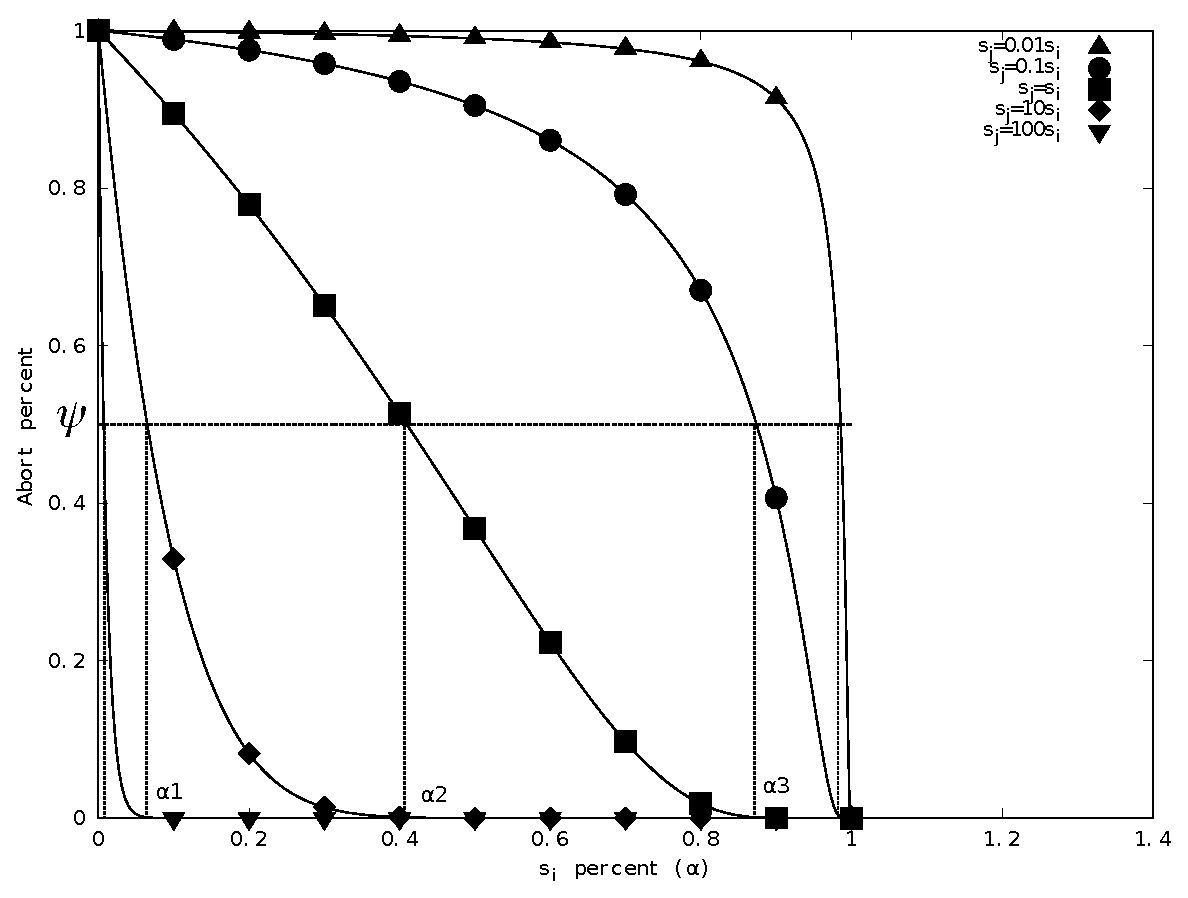
\includegraphics[scale=0.4]{figures/figure16}
\caption{\label{fig16}Interference of $s_{i}^{k}$ by various lengths of 
$s_{j}^{l}$}
\end{figure}

The behavior of LCM is illustrated in Figure~\ref{fig16}. In this figure, the horizontal axis corresponds to different values of $\alpha$ ranging from $0$ to $1$, and the vertical axis corresponds to different values of abort opportunities, $f(c_{ij}^{kl},\alpha)$, ranging from $0$ to $1$ and calculated by~(\ref{eq49}):
\begin{equation}
f(c_{ij}^{kl},\alpha)=e^{\frac{-c_{ij}^{kl}\alpha}{1-\alpha}}
\label{eq49}\end{equation}
where $c_{ij}^{kl}$ is calculated by~(\ref{cm_eq}).

Figure~\ref{fig16} shows one atomic section $s_i^k$ (whose $\alpha$ changes along the horizontal axis) interfered by five different lengths of $s_j^l$.
For a predefined value of $f(c_{ij}^{kl},\alpha)$ (denoted as $\psi$ in Algorithm~\ref{alg_lcm}), there corresponds a specific value of $\alpha$ (which is $\alpha_{ij}^{kl}$ in Algorithm~\ref{alg_lcm}) for each curve. For example, when $len(s_j^l)=0.1 \times len(s_i^k)$, $s_j^l$ aborts $s_i^k$ if the latter has not executed more than $\alpha3$ percentage (shown in Figure~\ref{fig16}) of its execution length. As $len(s_{j}^{l})$ decreases, the corresponding $\alpha_{ij}^{kl}$ increases (as shown in Figure~\ref{fig16}, $\alpha3>\alpha2>\alpha1$).

Equation (\ref{eq49}) achieves the desired requirement that the abort opportunity is reduced as $s_{i}^{k}$ gets closer to the end of its execution (as $\alpha\rightarrow1,\, f(c_{ij}^{kl},1)\rightarrow0$),
or as the length of the conflicting transaction increases (as $c_{ij}^{kl}\rightarrow\infty,\, f(\infty,\alpha)\rightarrow0$). Meanwhile, this abort opportunity is increased as $s_{i}^{k}$ is interfered closer to its release (as $\alpha\rightarrow0,\, f(c_{ij}^{kl},0)\rightarrow1$),
or as the length of the conflicting transaction decreases (as $c_{ij}^{kl}\rightarrow0,\, f(0,\alpha)\rightarrow1$).

LCM is not a centralized CM, which means that, upon a conflict, each transactions has to decide whether it must commit or abort. LCM suffers from transitive retry (Section~\ref{subsec:ecm_transitive_retry}).
%
\begin{clm}\label{clm:lcm-transitive-retry}
LCM suffers from transitive retry for multi-object transactions.
\end{clm}
%
\begin{proof}\normalfont
%
Following the proof of Claim~\ref{ecm-rcm-transitive-retry}, Claim follows.
%
\end{proof}
%
\subsection{LCM Illustrative Example}
%
Behaviour of LCM can be illustrated by the following example:
\begin{itemize}
\item Transaction $s_{i}^{k}\in\tau_{i}^{x}$ begins execution.
Currently, $s_{i}^{k}$ does not conflict with any other transaction.
\item Transaction $s_{j}^{l}\in\tau_{j}^{y}$ is released while
$s_{i}^{k}$ is still running. $\Theta_i^{k^{ex}} \cap \Theta_j^l \neq \emptyset$ and $p_{j}^{y}>p_{i}^{x}$ (where priority is dynamic in G-EDF, and fixed in G-RMA). $c_{ij}^{kl}$,
$\alpha_{ij}^{kl}$ and $\alpha$ are calculated by steps~\ref{step_cijkl} to~\ref{step_alpha} 
in Algorithm~\ref{alg_lcm}. $s_{i}^{k}$ has not reached $\alpha$
percentage of its execution length yet. 
\item $\alpha<\alpha_{ij}^{kl}$. Then, $s_{j}^{l}$ is allowed
to abort and restart $s_{i}^{k}$.
\item $s_{j}^{l}$ commits. $s_{i}^{k}$ executes again.
\item Transaction $s_{h}^{v}\in\tau_{h}^{u}$ is released while
$s_{i}^{k}$ is running. $\Theta_i^{k^{ex}} \cap \Theta_h^v \neq \emptyset$ and $p_{h}^{u}>p_{i}^{x}$. $c_{ih}^{kv}$,
$\alpha_{ih}^{kv}$ and $\alpha$ are calculated by steps~\ref{step_cijkl} to~\ref{step_alpha}
in Algorithm~\ref{alg_lcm}. $s_{i}^{k}$ has already passed $\alpha$
percentage of its execution length. So, $s_{h}^{v}$ aborts
and restarts in favour of $s_{i}^{k}$.
\item Transaction $s_{a}^{b}\in\tau_{a}^{f}$ is released. $\Theta_i^{k^{ex}} \cap \Theta_a^b \neq \emptyset$ and $p_{a}^{f}>p_{i}^{x}$
but $p_{a}^{f}<p_{h}^{u}$. $c_{ia}^{kb}$, $\alpha_{ia}^{kb}$
and $\alpha$ are calculated by steps~\ref{step_cijkl} to~\ref{step_alpha} in Algorithm~\ref{alg_lcm}.
$s_{i}^{k}$ has not reached $\alpha$ percentage of its execution
length yet. So, $s_{a}^{b}$ is allowed to abort $s_{i}^{k}$.
Because $s_{a}^{b}$ is just starting, LCM allows $s_{h}^{v}$
to abort $s_{a}^{b}$. So, the highest priority transaction
is not blocked by an intermediate priority transaction $s_{a}^{b}$.
\item When $s_{h}^{v}$ commits. $s_{a}^{b}$ is allowed
to execute while $s_{i}^{k}$ is retrying.
\item When $s_{a}^{b}$ commits, $s_{i}^{k}$ executes.
\item Transaction $s_{c}^{n}\in\tau_{o}^{z}$ is released while
$s_{i}^{k}$ is running. $\Theta_i^{k^{ex}} \cap \Theta_c^n \neq \emptyset$ and $p_{o}^{z}<p_{i}^{x}$. So, $s_{i}^{k}$
commits first, then $s_{c}^{n}$ is allowed to proceed.
\end{itemize} 
%
\section{Properties}\label{sec:lcm_properties}
%
LCM properties are given by the following Lemmas. These properties are used to derive retry cost and response time of transactions and tasks under LCM.
%
\begin{clm}\label{clm:lcm_deadlock_avoid}
%
$r\left(s_i^k\right)$ is updated each time $s_i^k$ aborts and retries to the new start time of the new retry to avoid deadlock that can result from conflicting transactions aborting each other.
%
\end{clm}
%
\begin{proof}
%
Assume a set of transactions $S$ that are conflicting together. Each transaction aborts and retries due to the others. So, a higher priority transaction $s_j^l$ aborts and retries due to a lower priority transaction $s_i^k$. $s_i^k$ itself aborts and retries due to another transaction. Thus, the new $r\left(s_i^k\right)$ will be at least equal to the new $r\left(s_j^l\right)$. By definition of LCM, $s_j^l$ will be chosen to commit first because of its higher priority. By extending this result to all transactions in $S$, the highest priority transaction will commit. Thus, deadlock is avoided. Claim follows.
%
\end{proof}
%
\begin{clm}\label{LCM_higher_rc}
%
Let $s_{j}^{l}$ interferes once with $s_{i}^{k}$ at most at $\alpha_{ij}^{kl}$. $p\left(s_j^l\right) > p\left(s_i^k\right)$. Then, the maximum contribution of $s_{j}^{l}$ to 
$s_{i}^{k}$'s retry cost is:
\begin{equation}
W_i^k(s_j^l)\le \alpha_{ij}^{kl}len\Big(s_{i}^{k}\Big)+len\Big(s_{j}^{l}\Big)\label{eq47}\end{equation}
%
\end{clm}
%
\begin{proof}\normalfont
%
If $s_{j}^{l}$ interferes with $s_{i}^{k}$ at a $\Upsilon$ percentage, where $\Upsilon<\alpha_{ij}^{kl}$,
then the retry cost of $s_{i}^{k}$ is $\Upsilon len(s_{i}^{k})+len(s_{j}^{l})$, which is lower than that calculated in (\ref{eq47}). Besides, 
if $s_{j}^{l}$ interferes with $s_{i}^{k}$ after
$\alpha_{ij}^{kl}$ percentage, then $s_{i}^{k}$ will not
abort.
%
\end{proof}
%
\begin{clm}\label{LCM_lower_rc}
%
A higher priority transaction, $s_j^l$, aborts and retries due to a lower priority transaction, $s_i^k$, if $s_{j}^{l}$ interferes with $s_{i}^{k}$ after the $\alpha_{ij}^{kl}$ percentage. $s_j^l$'s retry cost, due to $s_{i}^{k}$ is upper bounded by:
%
\begin{equation}
W_j^l(s_i^k)\le \Big(1-\alpha_{ij}^{kl}\Big)len\Big(s_{i}^{k}\Big)
\label{eq48}
\end{equation}
%
\end{clm}
%
\begin{proof}\normalfont
It is derived directly from Claim~\ref{LCM_higher_rc}, as $s_j^l$ will have to retry for the remaining length of $s_i^k$.
\end{proof}
%
\begin{clm}\label{clm:alpha_increase_with_max_interfered}
As length of $s_i^k$, interfered by a higher priority transaction $s_j^l$, increases, then $\alpha_{ij}^{kl}$ also increases.
\end{clm}
%
\begin{proof}\normalfont
%
As $len\left(s_i^k\right)$ increases, then $c_{ij}^{kl}$ decreases by definition of (\ref{cm_eq}). Noting that $ln(\Psi) \le 0$ because $\Psi \in [0,1]$. Thus, (\ref{eq49}) increases as $c_{ij}^{kl}$ decreases. $\alpha_{ij}^{kl}$ is calculated by (\ref{eq49}). Claim follows.
%
\end{proof}
%
\begin{clm}\label{clm:lcm_effect_one_tx_in_rc_multiple_txs}
%
Let $conf\left\{ s_{i}^{k}\right\} $ be the set of all transactions
that do not belong to any job of $\tau_{i}$ and are conflicting, directly or indirectly(transitively), with
$s_{i}^{k}$. Each transaction $s_{j}^{l}\in conf\left\{ s_{i}^{k}\right\},\,p\left(s_j^l\right)>p\left(s_i^k\right) $
contributes to the retry cost of $s_{i}^{k}$ by at most 
\begin{equation}
len\left(s_{j}^{l}+\alpha_{max}^{jl}s_{max}^{jl}(\Theta)\right)\label{eq:lcm_effect_one_tx_in_rc_multiple_txs}
\end{equation}
where $s_{max}^{jl}(\Theta)$ is the maximum length atomic section
(transaction) in $conf\{s_{i}^{k}\}$ that accesses at least one object in $\Theta$ and its priority is lower than $p(s_{j}^{l})$. $s_{max}^{jl} \not\in s_{j}$ and $\Theta\subseteq\Theta_{i}^{k^{ex}}\cap\Theta_{j}^{l}$.
%
\end{clm}
%
\begin{proof}
Under ECM and RCM (Chapter~\ref{ecm-rcm}), lower priority transactions abort and retry only due to higher priority transactions. Whereas, under LCM, a transaction $s_i^k$ can be aborted due to higher priority transactions. $s_i^k$ can also be delayed by lower priority transactions. Thus, proof follows proof of Claim~\ref{clm:effect_one_tx_in_rc_multiple_txs} with the following modifications:
\begin{compactitem}
\item According to Claims~\ref{LCM_higher_rc} and~\ref{LCM_lower_rc}, $s_j^l$ can cause lower priority transactions to retry and higher priority transactions to be delayed. From Claims~\ref{LCM_higher_rc} and~\ref{LCM_lower_rc}, it appears that contribution of $s_j^l$ to the retry cost of lower priority transactions is greater than delay caused by $s_j^l$ to higher priority transactions. Thus, retry cost caused by $s_j^l$ to lower priority transactions is taken as the contribution of $s_j^l$ to the retry cost of $s_i^k$.
\item By Claim~\ref{clm:alpha_increase_with_max_interfered} and definition of $s_{max}^{jl}\left(\Theta\right)$, $\alpha_{max}^{jl}$ is the maximum $\alpha$ that results from interference of a lower priority transaction- accessing any object $\theta \in \Theta$ - by $s_j^l$.
\item $s_i^k$ can abort and retry due to higher priority transactions. Also, $s_i^k$ can be delayed due to lower priority transactions. Thus, $p\left(s_{max}^{jl}\right)<p\left(s_j^l\right)$, but $p\left(s_{max}^{jl}\right)$ does not have to be greater than $p\left(s_i^k\right)$.
\end{compactitem}
Claim follows.
%
\end{proof}
%NEW_VERSION
\begin{clm}
\label{no priority inversion in lcm}
%
A higher priority job, $\tau_j^y$, suffers from priority inversion for at most number of atomic sections in $\tau_j^y$.
\end{clm}
%
\begin{proof}\normalfont
Assuming three atomic sections, $s_i^k \in \tau_i^x$, $s_j^l \in \tau_j^y$ and $s_a^b \in \tau_a^z$. $p\left(s_j^l\right) > p\left(s_i^k\right)$ and $s_j^l$ interferes with $s_i^k$ after $\alpha_{ij}^{kl}$. Then $s_j^l$ will have to abort and retry. At this time, if $s_a^b$ interferes with the other two atomic sections, then $s\left(s_i^k\right) < s\left(s_j^l\right) < s\left(s_a^b\right)$, and the LCM is to decide which transaction to commit based on comparison between each two transactions. So, we have the following cases:-
\begin{itemize}
\item $p\left(s_a^b\right) < p\left(s_i^k\right) < p\left(s_j^l\right)$, then $s_a^b$ will not abort any one because $s_a^b$ starts after the other two transactions and $s_a^b$ has the lowest priority. So. $\tau_j$ is not blocked by $\tau_a$.
\item $p\left(s_i^k\right) < p\left(s_a^b\right) < p\left(s_j^l\right)$. If $s_a^b$ interferes with $s_i^k$ before $\alpha_{ia}^{kb}$, then $s_a^b$ is allowed to abort $s_i^k$. Comparison between $s_j^l$ and $s_a^b$ will result in LCM choosing $s_j^l$ to commit and abort $s_a^b$ starts after $s_j^l$, and $p\left(s_j^l\right) > p\left(s_a^b\right)$. So, the higher priority job $\tau_j^y$ is not blocked by the intermediate priority job $\tau_a^z$. If $s_a^b$ is not allowed to abort $s_i^k$, the situation is still the same, because $s_j^l$ was already retrying until $s_i^k$ finishes. When $s_i^k$ finishes, LCM will still choose the higher priority $s_j^l$.
\item $p\left(s_a^b\right) > p\left(s_j^l\right) > p\left(s_i^k\right)$, then if $s_a^b$ is chosen to commit, this is not priority inversion for $\tau_j^y$ because $\tau_a^z$ is of higher priority.
\item if $\tau_a^z$ preempts $\tau_i^x$, then LCM will compare only between $s_j^l$ and $s_a^b$. If $p\left(s_a^b\right)<p\left(s_j^l\right)$, then $s_j^l$ will commit because of its job's higher priority. Otherwise, $s_j^l$ will retry, but this will not be priority inversion because $\tau_a^z$ is already of higher priority than $\tau_j^y$. If $\tau_a^z$ does not access any object but it preempts $\tau_i^x$, then LCM will choose $s_j^l$ to commit as only already running transactions are competing together.
\end{itemize}
So, by generalizing these cases to any number of conflicting jobs, it is seen that when an atomic section, $s_j^l$, of a higher priority job is in conflict with a number of atomic sections belonging to lower priority jobs, $s_j^l$ can suffer from priority inversion by only one of them. After that, LCM will choose $s_j^l$ before other lower priority transactions. So, each higher priority job can suffer priority inversion at most its number of atomic section. Claim follows.
\end{proof}
%
\begin{clm}
\label{max_pri_inv}
The maximum delay suffered by $s_j^l(\theta)$ due to lower priority jobs is caused by the maximum length atomic section accessing object $\theta$, which belongs to a lower priority job than $\tau_j^b$ that owns $s_j^l(\theta)$.
\end{clm}

\begin{proof}\normalfont
Assume three atomic sections, $s_i^k(\theta)$, $s_j^l(\theta)$, and $s_h^z(\theta)$, where $p_j>p_i$, $p_j>p_h$, and $len(s_i^k(\theta))>len(s_h^z(\theta))$. Now, $\alpha_{ij}^{kl}>\alpha_{hj}^{zl}$ and $c_{ij}^{kl}<c_{hj}^{zl}$. By applying~(\ref{eq48}) to obtain the contribution of $s_i^k(\theta)$ and $s_h^z(\theta)$ to the priority inversion of $s_j^l(\theta)$ and dividing them, we get:
\begin{eqnarray*}
\frac{W_{j}^{l}(s_{i}^{k}(\theta))}{W_{j}^{l}(s_{h}^{z}(\theta))} & = & \frac{\left(1-\alpha_{ij}^{kl}\right)len(s_{i}^{k}(\theta))}{\left(1-\alpha_{hj}^{zl}\right)len(s_{h}^{z}(\theta))}
\end{eqnarray*}
By substitution for $\alpha$s from~(\ref{eq49}):
\begin{eqnarray*}
 & = & \frac{(1-\frac{ln\psi}{ln\psi-c_{ij}^{kl}})len(s_{i}^{k}(\theta))}{(1-\frac{ln\psi}{ln\psi-c_{hj}^{zl}})len(s_{h}^{z}(\theta))}
  =  \frac{(\frac{-c_{ij}^{kl}}{ln\psi-c_{ij}^{kl}})len(s_{i}^{k}(\theta))}{(\frac{-c_{hj}^{zl}}{ln\psi-c_{hj}^{zl}})len(s_{h}^{z}(\theta))}\end{eqnarray*}
$\because ln\psi \le 0$ and $c_{ij}^{kl},c_{hj}^{kl} > 0, \therefore$ by substitution from~(\ref{cm_eq})
\begin{eqnarray*}
 & = & \frac{len(s_{j}^{l}(\theta))/(ln\psi-c_{ij}^{kl})}{len(s_{j}^{l}(\theta))/(ln\psi-c_{hj}^{zl})}
  =  \frac{ln\psi-c_{hj}^{zl}}{ln\psi-c_{ij}^{kl}}>1\end{eqnarray*}
Thus, as the length of the interfered atomic section increases, the delay suffered by the interfering atomic section increases. Claim follows.
\end{proof}


\section{\label{response g-edf/lcm}Response Time of G-EDF/LCM}

%Toward establishing the response time under G-EDF/LCM, we introduce a set of Claims.

\begin{clm}\label{GEDF/LCM response time}
$RC(T_i)$ for a task $\tau_i$ under G-EDF/LCM is upper bounded by:

\begin{eqnarray}
RC(T_i) & = & \Bigg(\sum_{\forall \tau_h \in \gamma_i}\sum_{\forall\theta \in \theta_i \wedge \theta_h}\Bigg(\left\lceil\frac{T_{i}}{T_{h}}\right\rceil\sum_{\forall s_{h}^{l}(\theta)}len\Big(s_{h}^{l}(\theta)\Big)\nonumber\\
& + & \alpha_{max}^{hl}len\Big(s_{max}^{h}(\theta)\Big)\Bigg)\Bigg) + \sum_{\forall s_{i}^{y}(\theta)}\left(1-\alpha_{max}^{iy}\right)len\left(s_{max}^i(\theta)\right)  
\label{eq78}\end{eqnarray}

where $\alpha_{max}^{hl}$ is the $\alpha$ value that corresponds to $\psi$ due to the interference of $s_{max}^h(\theta)$ by $s_h^l(\theta)$. $\alpha_{max}^{iy}$ is the $\alpha$ value that corresponds to $\psi$ due to the interference of $s_{max}^i(\theta)$ by $s_i^y(\theta)$.
\end{clm}

\begin{proof}\normalfont
The maximum number of higher priority instances of $\tau_h$ that can interfere with $\tau_i^x$ is $\left\lceil\frac{T_i}{T_h}\right\rceil$, as shown in Figure~\ref{fig17}, where one instance of $\tau_h$ and $\tau_h^p$ coincides with the absolute deadline of $\tau_i^x$.

By using Claims~\ref{gedf-edf},~\ref{LCM_higher_rc},~\ref{LCM_lower_rc},~\ref{no priority inversion in lcm} and~\ref{max_pri_inv} to determine the effect of atomic sections belonging to higher and lower priority instances of interfering tasks to $\tau_i^x$, Claim follows.
\end{proof}


Response time of $\tau_{i}$ is calculated by~(\ref{eq10}).
\begin{figure}
\begin{centering}
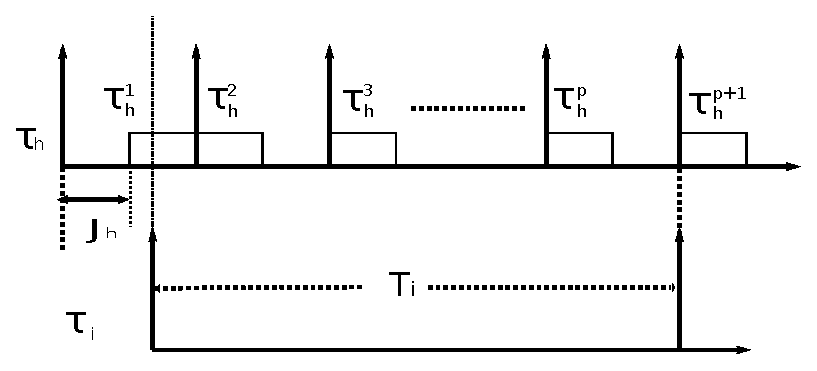
\includegraphics[scale=0.6]{figures/figure18}
\par\end{centering}
\caption{\label{fig17}$\tau_h^p$ has a higher priority than $\tau_i^x$}
\end{figure}

\section{Schedulability of G-EDF/LCM}
\label{performance g-edf-lcm}
We now compare the schedulability of G-EDF/LCM with ECM (Chapter~\ref{ecm-rcm}) to understand when G-EDF/LCM will perform better. 
Toward this, we compare the total utilization of ECM with that of G-EDF/LCM. For each method, we inflate the $c_i$ of each task $\tau_i$ by adding the retry cost suffered by $\tau_i$. Thus, if method $A$ adds retry cost $RC_A(T_i)$ to $c_i$, and method $B$ adds retry cost $RC_B(T_i)$ to $c_i$, then the schedulability of $A$ and $B$ are compared as:
\begin{eqnarray}
\sum_{\forall \tau_{i}}\frac{c_{i}+RC_A(T_{i})}{T_{i}} & \le & \sum_{\forall \tau_{i}}\frac{c_{i}+RC_B(T_{i})}{T_{i}}\nonumber\\
\sum_{\forall \tau_{i}}\frac{RC_A(T_{i})}{T_{i}} & \le & \sum_{\forall \tau_{i}}\frac{RC_B(T_{i})}{T_{i}}
\label{eqa}\end{eqnarray}
Thus, schedulability is compared by substituting the retry cost added by the synchronization methods in (\ref{eqa}).

\subsection{Schedulability of G-EDF/LCM and ECM}
\begin{clm}\label{lcm versus ecm}
Let $s_{max}$ be the maximum length atomic section accessing any object $\theta$. Let $\alpha_{max}$ and $\alpha_{min}$ be the maximum and minimum values of $\alpha$ for any two atomic sections $s_i^k(\theta)$ and $s_j^l(\theta)$. Given a threshold $\psi$, schedulability of G-EDF/LCM is equal or better than ECM if for any task $\tau_i$:
\begin{equation}
\frac{1-\alpha_{min}}{1-\alpha_{max}} \le \sum_{\forall \tau_h \in \gamma_i}\left\lceil\frac{T_i}{T_h}\right\rceil
\label{edf-lcm-ecm}\end{equation}
\end{clm}

\begin{proof}\normalfont
Under ECM, $RC(T_{i})$ is upper bounded by:
\begin{equation}
RC(T_{i})\le\sum_{\forall \tau_{h}\in\gamma_{i}}\sum_{\forall \theta\in\ (\theta_{i}\wedge\theta_{h})}\left(\left\lceil\frac{T_{i}}{T_{h}}\right\rceil\sum_{\forall s_{h}^{z}(\theta)}2len(s_{max})\right)\label{eq61}\end{equation}
with the assumption that all lengths of atomic sections of (\ref{eq3}), (\ref{eq4}) and~(\ref{eq78}) are replaced by $s_{max}$.
%~\cite{stmconcurrencycontrol:emsoft11}. 
Let $\alpha_{max}^{hl}$ in~(\ref{eq78}) be replaced with $\alpha_{max}$, and $\alpha_{max}^{iy}$ in~(\ref{eq78}) be replaced with $\alpha_{min}$. 
As $\alpha_{max}$, $\alpha_{min}$, and $len(s_{max})$ are all constants, (\ref{eq78}) is upper bounded by:
\begin{eqnarray}
RC(T_i) & \le & \Bigg(\sum_{\forall \tau_h \in \gamma_i}\sum_{\forall\theta \in \theta_i \wedge \theta_h}\Bigg(\left\lceil\frac{T_{i}}{T_{h}}\right\rceil\sum_{\forall s_{h}^{l}(\theta)}\left(1+\alpha_{max}\right)\nonumber\\
& & len\Big(s_{max}\Big)\Bigg)\Bigg)
 +  \sum_{\forall s_{i}^{y}(\theta)}\Big(1-\alpha_{min}\Big)len\Big(s_{max}\Big)\nonumber\\ 
\label{eq101}\end{eqnarray}

If $\beta_1^{ih}$ is the total number of times any instance of $\tau_h$ accesses shared objects with $\tau_i$, then $\beta_1^{ih}=\sum_{\forall \theta\in(\theta_{i}\wedge\theta_{h})}\sum_{\forall s_{h}^{z}(\theta)}$. Furthermore, if $\beta_2^i$ is the total number of times any instance of $\tau_i$ accesses shared objects with any other instance,   $\beta_2^i=\sum_{\forall s_{i}^{y}(\theta)}$\textit{, where $\theta$ is shared with another task}. Then, $\beta_{i}=max\{max_{\forall \tau_h \in \gamma_i}\{\beta_1^{ih}\},\beta_2^i\}$ is the maximum number of accesses to all shared objects by any instance of $\tau_{i}$ or $\tau_{h}$. 
Thus, (\ref{eq61}) becomes:
\begin{equation}
RC(T_{i})\le\sum_{\tau_{h}\in\gamma_{i}}2\left\lceil\frac{T_{i}}{T_{h}}\right\rceil\beta_{i}len(s_{max})
\label{eq63}\end{equation}
and (\ref{eq101}) becomes:
%\begin{eqnarray}
%RC(T_{i}) & \le & \beta_{i}len(s_{max}) \Bigg((1-\alpha_{min})\nonumber\\
%& + & \sum_{\forall \tau_h \in \gamma_i}\left\lceil\frac{T_{i}}{T_{h}}\right\rceil(1+\alpha_{max})\Bigg)
%\label{eq102}\end{eqnarray}

\begin{equation}
RC(T_{i}) \le \beta_{i}len(s_{max}) \left((1-\alpha_{min}) + \sum_{\forall \tau_h \in \gamma_i}\left\lceil\frac{T_{i}}{T_{h}}\right\rceil(1+\alpha_{max})\right)
\label{eq102}\end{equation}

We can now compare the total utilization of G-EDF/LCM with that of ECM by comparing~(\ref{eq101}) and~(\ref{eq102}) for all $\tau_i$:
\begin{eqnarray}
& & \sum_{\forall \tau_{i}}\frac{(1-\alpha_{min})+\sum_{\forall \tau_{h}\in\gamma_{i}}\left(\left\lceil\frac{T_{i}}{T_{h}}\right\rceil(1+\alpha_{max})\right)}{T_{i}} \nonumber\\
& \le &   \sum_{\forall \tau_{i}}\frac{\sum_{\forall \tau_{h}\in\gamma_{i}}2\left\lceil\frac{T_{i}}{T_{h}}\right\rceil}{T_{i}}\label{eqc}\end{eqnarray}

(\ref{eqc}) is satisfied if for each $\tau_{i}$, the following condition is satisfied:
\begin{equation*}
(1-\alpha_{min})+\sum_{\forall \tau_h \in \gamma_i}\left(\left\lceil\frac{T_{i}}{T_{h}}\right\rceil(1+\alpha_{max})\right)  \le  2\sum_{\forall \tau_h \in \gamma_i}\left\lceil\frac{T_{i}}{T_{h}}\right\rceil
\end{equation*}
\begin{equation*}
\therefore\frac{1-\alpha_{min}}{1-\alpha_{max}}  \le  \sum_{\forall \tau_h \in \gamma_i}\left\lceil\frac{T_{i}}{T_{h}}\right\rceil
\end{equation*}
Claim follows.
\end{proof}


\subsection{G-EDF/LCM versus Lock-free}
\label{gedf-lcm-lock-free}
We consider the retry-loop lock-free synchronization for G-EDF given in~\cite{key-5}. This lock-free approach is the most relevant to our work. 

\begin{clm}\label{gedf-lcm-lock-free_clm} 
Let $s_{max}$ denote $len(s_{max})$ and $r_{max}$ denote the maximum execution cost of a single iteration of any retry loop of any task in the retry-loop lock-free algorithm in~\cite{key-5}. Now, G-EDF/LCM achieves higher schedulability than the retry-loop lock-free approach if the upper bound on $s_{max}/r_{max}$ under G-EDF/LCM ranges between 0.5 and 2 (which is higher than that under  ECM). 
\end{clm}

\begin{proof}\normalfont
From~\cite{key-5}, the retry-loop lock-free algorithm
is upper bounded by: 
\begin{equation}
RL(T_{i})=\sum_{\tau_{h}\in\gamma_{i}}\left(\left\lceil \frac{T_{i}}{T_{h}}\right\rceil +1\right)\beta_{i}r_{max}\label{eq32-1}
\end{equation}
 where $\beta_{i}$ is as defined in Claim~\ref{lcm versus ecm}.
The retry cost of $\tau_{i}$ in G-EDF/LCM is upper bounded by (\ref{eq102}).
By comparing G-EDF/LCM's total utilization with that of the retry-loop
lock-free algorithm, we get: 
\begin{eqnarray*}
 & \sum_{\forall\tau_{i}}\frac{\left((1-\alpha_{min})+\sum_{\forall\tau_{h}\in\gamma_{i}}\left(\left\lceil \frac{T_{i}}{T_{h}}\right\rceil (1+\alpha_{max})\right)\right)\beta_{i}s_{max}}{T_{i}}\\
\le & \sum_{\forall\tau_{i}}\frac{\sum_{\forall\tau_{h}\in\gamma_{i}}\left(\left\lceil \frac{T_{i}}{T_{h}}\right\rceil +1\right)\beta_{i}r_{max}}{T_{i}}
\end{eqnarray*}
 
\begin{eqnarray}
\therefore\frac{s_{max}}{r_{max}}\le\frac{\sum_{\forall\tau_{i}}\frac{\sum_{\forall\tau_{h}\in\gamma_{i}}\left(\left\lceil \frac{T_{i}}{T_{h}}\right\rceil +1\right)\beta_{i}}{T_{i}}}{\sum_{\forall\tau_{i}}\frac{\left((1-\alpha_{min})+\sum_{\forall\tau_{h}\in\gamma_{i}}\left(\left\lceil \frac{T_{i}}{T_{h}}\right\rceil (1+\alpha_{max})\right)\right)\beta_{i}}{T_{i}}}\label{u-gedf-lcm-ecm}
\end{eqnarray}


Let the number of tasks that have shared objects with $\tau_{i}$
be $\omega$ (i.e., $\sum_{\tau_{h}\in\gamma_{i}}=\omega\ge1$ since
at least one task has a shared object with $\tau_{i}$; otherwise,
there is no conflict between tasks). Let the total number of tasks
be $n$, so $1\le\omega\le n-1$, and $\left\lceil \frac{T_{i}}{T_{h}}\right\rceil \in[1,\infty[$.
To find the minimum and maximum values for the upper bound on $s_{max}/r_{max}$,
we consider the following cases: 
\begin{itemize}
\item $\alpha_{min}\rightarrow0,\alpha_{max}\rightarrow0$ 
\end{itemize}
$\therefore$~(\ref{u-gedf-lcm-ecm}) will be: 
\begin{eqnarray}
\frac{s_{max}}{r_{max}} & \le & 1+\frac{\sum_{\forall\tau_{i}}\frac{\omega-1}{T_{i}}}{\sum_{\forall\tau_{i}}\frac{1+\sum_{\forall\tau_{h}\in\gamma_{i}}\left\lceil \frac{T_{i}}{T_{h}}\right\rceil }{T_{i}}}\nonumber \\
\label{s-r-1}
\end{eqnarray}
 By substituting the edge values for $\omega$ and $\left\lceil \frac{T_{i}}{T_{h}}\right\rceil $
in~(\ref{s-r-1}), we derive that the upper bound on $s_{max}/r_{max}$
lies between 1 and 2.
\begin{itemize}
\item $\alpha_{min}\rightarrow0,\alpha_{max}\rightarrow1$ 
\end{itemize}
(\ref{u-gedf-lcm-ecm}) becomes 
\begin{eqnarray}
\frac{s_{max}}{r_{max}} & \le & 0.5+\frac{\sum_{\forall\tau_{i}}\frac{\omega-0.5}{T_{i}}}{\sum_{\forall\tau_{i}}\frac{1+2\sum_{\forall\tau_{h}\in\gamma_{i}}\left\lceil \frac{T_{i}}{T_{h}}\right\rceil }{T_{i}}}\label{s-r-2}
\end{eqnarray}
 By applying the edge values for $\omega$ and $\left\lceil \frac{T_{i}}{T_{h}}\right\rceil $
in~(\ref{s-r-2}), we derive that the upper bound on $s_{max}/r_{max}$
lies between 0.5 and 1.
\begin{itemize}
\item $\alpha_{min}\rightarrow1,\alpha_{max}\rightarrow0$ 
\end{itemize}
This case is rejected since $\alpha_{min}\le\alpha_{max}$.
\begin{itemize}
\item $\alpha_{min}\rightarrow1,\alpha_{max}\rightarrow1$ 
\end{itemize}
$\therefore$~(\ref{u-gedf-lcm-ecm}) becomes: 
\begin{eqnarray}
\frac{s_{max}}{r_{max}} & \le & 0.5+\frac{\sum_{\tau_{i}}\frac{\omega}{T_{i}}}{2\sum_{\tau_{i}}\frac{\sum_{\forall\tau_{h}\in\gamma_{i}}\left\lceil \frac{T_{i}}{T_{h}}\right\rceil }{T_{i}}}\label{s-r-4}
\end{eqnarray}
 By applying the edge values for $\omega$ and $\left\lceil \frac{T_{i}}{T_{h}}\right\rceil $
in~(\ref{s-r-4}), we derive that the upper bound on $s_{max}/r_{max}$
lies between 0.5 and 1, which is similar to that achieved by ECM.

Summarizing from the previous cases, the upper bound on $s_{max}/r_{max}$
lies between 0.5 and 2, whereas for ECM,
it lies between 0.5 and 1. Claim follows.

\end{proof}

\section{Response Time of G-RMA/LCM}
\label{rma}

\begin{clm}\label{response g-rma/lcm}
Let $\lambda_{2}(j,\theta)=\sum_{\forall s_{j}^{l}(\theta)}len(s_{j}^{l}(\theta))+\alpha_{max}^{jl}len(s_{max}^{j}(\theta))$, where $\alpha_{max}^{jl}$ is the $\alpha$ value corresponding to $\psi$ due to the interference of $s_{max}^j(\theta)$ by $s_j^l(\theta)$. The retry cost of any task $\tau_i$ under G-RMA/LCM during $T_i$ 
is given by:
%\begin{eqnarray}
%RC\left(T_i\right) & = &
%  \sum_{\forall \tau_{j}^{*}}\left(\sum_{\theta\in(\theta_{i}\wedge\theta_{j})}\left(\left(\left\lceil\frac{T_i}{T_{j}}\right\rceil +1\right)\lambda_{2}(j,\theta)\right)\right)\nonumber\\
%& + & \sum_{\forall s_{i}^{y}(\theta)}\Big(1-\alpha_{max}^{iy}\Big)len\Big(s_{max}^i(\theta)\Big)
%\label{eq60}
%\end{eqnarray}
\begin{equation}
RC\left(T_i\right) = \sum_{\forall\tau_{j}^{*}}\left(\sum_{\theta\in(\theta_{i}\wedge\theta_{j})}\left(\left(\left\lceil\frac{T_i}{T_{j}}\right\rceil +1\right)\lambda_{2}(j,\theta)\right)\right) + \sum_{\forall s_{i}^{y}(\theta)}\left(1-\alpha_{max}^{iy}\right)len\left(s_{max}^i(\theta)\right)
\label{eq60}
\end{equation}

where $\tau_{j}^{*}=\{\tau_{j}|(\tau_{j}\in\gamma_{i})\wedge(p_{j}>p_{i})\}$.
\end{clm}

\begin{proof}\normalfont
Under G-RMA, all instances of a higher priority task, $\tau_{j}$, can conflict with a lower priority task,
$\tau_{i}$, during $T_{i}$. (\ref{eq47}) can be used to determine the contribution of each conflicting atomic section in $\tau_j$ to $\tau_i$. Meanwhile, all instances of any task with lower priority than $\tau_{i}$ can conflict with $\tau_i$ during $T_{i}$. Claims~\ref{LCM_lower_rc} and~\ref{no priority inversion in lcm} can be used to determine the contribution of conflicting atomic sections in lower priority tasks to $\tau_i$.
%
  %over the whole $t(T_i)$ (unlike the case of G-EDF/LCM, where (\ref{eq59}) chooses which equation to use depending on whether or not $L$ is less than $\left\lfloor\frac{t(T_{i})-c_{h}}{t(T_{h})}\right\rfloor t(T_{h})+c_{h}$).
Using the previous notations and Claim~\ref{clm:rcm_retry_cost}, the Claim follows.
\end{proof}

The response time is calculated by~(\ref{eq22}) with replacing $RC(R_i^{up})$ with $RC(T_i)$.
%BR: You should say "..with $RC(T_i)$ replacing $RC(R_i^{up})$."

\section{Schedulability of G-RMA/LCM}
\label{rma eval}

\subsection{Schedulability of G-RMA/LCM and RCM}

\begin{clm}\label{rma_eval_clm}
Under the same assumptions of Claims~\ref{lcm versus ecm} and~\ref{response g-rma/lcm}, G-RMA/LCM's schedulability is equal or better than RCM if:
\begin{equation}
\frac{1-\alpha_{min}}{1-\alpha_{max}}\le \sum_{\forall \tau_j^*}\left( \left\lceil\frac{T_i}{T_j}\right\rceil +1 \right)
\label{eq70}\end{equation}
\end{clm}

\begin{proof}\normalfont
Under the same assumptions as that of Claims~\ref{lcm versus ecm} and~\ref{response g-rma/lcm}, (\ref{eq60}) can be upper bounded as:
%\begin{eqnarray}
%RC(T_i) & \le & \sum_{\forall \tau_{j}^{*}}\bigg(\left(\left\lceil\frac{T_{i}}{T_{j}}\right\rceil +1\right)(1+\alpha_{max})
% len(s_{max})\beta_{i}\bigg)\nonumber\\
% & + & (1-\alpha_{min})len(s_{max})\beta_{i}\label{eq68}\end{eqnarray}
\begin{equation}
RC(T_i) \le \sum_{\forall \tau_{j}^{*}}\left(\left(\left\lceil\frac{T_{i}}{T_{j}}\right\rceil +1\right)(1+\alpha_{max}) len(s_{max})\beta_{i}\right) + (1-\alpha_{min})len(s_{max})\beta_{i}\label{eq68}\end{equation} 
 
For RCM, (\ref{eq20}) for $RC(T_{i})$ is upper bounded by:
\begin{equation*}
RC(T_{i})\le\sum_{\forall \tau_{j}^{*}}\left(\left\lceil\frac{T_{i}}{T_{j}}\right\rceil +1\right)2\beta_{i}len(s_{max})\label{eq69}\end{equation*}\
By comparing the total utilization of G-RMA/LCM with that of RCM,
we get:
\begin{eqnarray}
 & \sum_{\forall\tau_{i}}\frac{len\left(s_{max}\right)\beta_{i}\left(\left(1-\alpha_{min}\right)+\sum_{\forall\tau_{j}^{*}}\left(\left(\left\lceil\frac{T_{i}}{T_{j}}\right\rceil+1\right)\left(1+\alpha_{max}\right)\right)\right)}{T_{i}}\nonumber\\
\le & \sum_{\forall\tau_{i}}\frac{2len\left(s_{max}\right)\beta_{i}\sum_{\forall\tau_{j}^{*}}\left(\left\lceil\frac{T_{i}}{T_{j}}\right\rceil+1\right)}{T_{i}}\label{grma-lcm-rcm}\end{eqnarray}
(\ref{grma-lcm-rcm}) is satisfied if $\forall \tau_i$~(\ref{eq70}) is satisfied. Claim follows.
\end{proof}


\subsection{G-RMA/LCM versus Lock-free}\label{g-rma lcm vs lock-free}

Although~\cite{key-5} considers retry-loop lock-free synchronization
for G-EDF systems,~\cite{key-5} also applies for G-RMA systems.

\begin{clm}\label{lcm rma lock-free comparison clm}

Let $s_{max}$ denote $len(s_{max})$ and $r_{max}$ denote the maximum
execution cost of a single iteration of any retry loop of any task
in the retry-loop lock-free algorithm in~\cite{key-5}. G-RMA/LCM
achieves higher schedulability than the retry-loop lock-free approach
if the upper bound on $s_{max}/r_{max}$ under G-RMA/LCM is no less
than 0.5. Upper bound on $s_{max}/r_{max}$ can extend to large values
when $\alpha_{min}$ and $\alpha_{max}$ are very large.

\end{clm}

\begin{proof}\normalfont

The retry cost for G-RMA/LCM is upper bounded by~(\ref{eq60}). Let $\gamma_{i}=\tau_{j}^{*}\cup\bar{\tau_{j}}$,
where $\tau_{j}^{*}$ is the set of higher priority tasks than $\tau_{i}$
sharing objects with $\tau_{i}$. $\bar{\tau_{j}}$ is the set
of lower priority tasks than $\tau_{i}$ sharing objects with
it. We follow the same definitions of $\beta_{i},\, r_{max}$, and
$RL(T_{i})$ given in the proof of Claim (\ref{gedf-lcm-lock-free_clm}).
Schedulability of G-RMA/LCM equals or exceeds the schedulability of retry-loop
lock-free algorithm if:
\begin{eqnarray}
\frac{s_{max}}{r_{max}} & \le & \frac{\sum_{\forall\tau_{i}}\frac{\sum_{\tau_{j}^{*}}\left(\left\lceil \frac{T_{i}}{T_{j}}\right\rceil +1\right)}{T_{i}}}{\sum_{\forall\tau_{i}}\frac{\Big(1-\alpha_{min}\Big)+\sum_{\tau_{j}^{*}}\left(\left\lceil \frac{T_{i}}{T_{j}}\right\rceil +1\right)\left(1+\alpha_{max}\right)}{T_{i}}}\nonumber\\
 & + & \frac{2\sum_{\forall\tau_{i}}\frac{\sum_{\forall\bar{\tau_{j}}}}{T_{i}}}{\sum_{\forall\tau_{i}}\frac{\Big(1-\alpha_{min}\Big)+\sum_{\tau_{j}^{*}}\left(\left\lceil \frac{T_{i}}{T_{j}}\right\rceil +1\right)\left(1+\alpha_{max}\right)}{T_{i}}}\nonumber\\
 & & \label{eq:lcm rma lock-free comparison 1} 
\end{eqnarray}
If $p_{j}<p_{i},\,\therefore\,\left\lceil \frac{T_{i}}{T_{j}}\right\rceil =1$, 
because the system assumes implicit deadline tasks and uses the G-RMA
scheduler. 
%
Let $\omega_{1}$ be the size of $\tau_i^*$ and $\omega_{2}$
be the size of $\bar{\tau_i}$. $\therefore$ $\omega_{1}^{i}\ge 1$ and $\omega_{2}^{i}\ge1$.
Otherwise, there is no conflict with $\tau_{i}$. To find the maximum
and minimum upper bounds for $s_{max}/r_{max}$, the following cases
are considered:
\begin{itemize}
\item $\alpha_{min}\rightarrow0,\,\alpha_{max}\rightarrow0$
\begin{equation}
\therefore\frac{s_{max}}{r_{max}}\le1+\frac{\sum_{\forall\tau_{i}}\frac{2\omega_{2}^{i}-1}{T_{i}}}{\sum_{\forall\tau_{i}}\frac{1+\sum_{\tau_{j}^{*}}\left(\left\lceil \frac{T_{i}}{T_{j}}\right\rceil +1\right)}{T_{i}}}\label{eq:lcm rma lock-free comparison 3}
\end{equation}
As the second term in (\ref{eq:lcm rma lock-free comparison 3}) is
always positive (because $\omega_{2}^{i}\ge1$), the minimum
upper bound on $s_{max}/r_{max}$ is $1$. To get the maximum upper
bound on $s_{max}/r_{max}$, let $\left\lceil \frac{T_{i}}{T_{j}}\right\rceil $
approach its minimum value of $1$, $\omega_{1}^{i}\rightarrow0$, and $\omega_{2}^{i}\rightarrow n-1$ 
(the maximum and minimum values for $\omega_{1}^{i}$ and $\omega_{2}^{i}$, 
respectively. $n$ is number of tasks). Now:
\[
\therefore\frac{s_{max}}{r_{max}}\le\left(2n-2\right)
\]
Of course, $n$ cannot be lower than $2$. Otherwise, there will be
no conflicting tasks.

\item $\alpha_{min}\rightarrow0,\,\alpha_{max}\rightarrow1$
\begin{equation}
\frac{s_{max}}{r_{max}}\le\frac{1}{2}+\frac{\sum_{\forall\tau_{i}}\frac{4\omega_{2}^{i}-1}{T_{i}}}{2\sum_{\forall\tau_{i}}\frac{1+2\sum_{\tau_{j}^{*}}\left(\left\lceil \frac{T_{i}}{T_{j}}\right\rceil +1\right)}{T_{i}}}\label{eq:lcm rma lock-free comparison 4}
\end{equation}
The minimum upper bound for $s_{max}/r_{max}$ is $0.5$. This can
happen when $T_{i}\gg T_{j}$. To get the maximum upper bound on $s_{max}/r_{max}$,
let $\left\lceil \frac{T_{i}}{T_{j}}\right\rceil $ approach its
minimum value $1$, $\omega_{2}^{i}\rightarrow n-1$, and $\omega_{1}^{i}\rightarrow0$. 
Now:
\[
\frac{s_{max}}{r_{max}}\le2n-2
\]

\item $\alpha_{min}\rightarrow1,\,\alpha_{max}\rightarrow0$
This case is rejected because $\alpha_{max}$ must be greater or equal
to $\alpha_{min}$.

\item $\alpha_{min}\rightarrow1,\,\alpha_{max}\rightarrow1$
\begin{equation}
\frac{s_{max}}{r_{max}}\le\frac{1}{2}+\frac{\sum_{\forall\tau_{i}}\frac{\omega_{2}^{i}}{T_{i}}}{\sum_{\forall\tau_{i}}\frac{\sum_{\tau_{j}^{*}}\left(\left\lceil \frac{T_{i}}{T_{j}}\right\rceil +1\right)}{T_{i}}}\label{eq:lcm rma lock-free comparison 5}
\end{equation}
The minimum upper bound for $s_{max}/r_{max}$ is $0.5$. This can
happen when $T_{i}\gg T_{j}$. To get the maximum upper bound on $s_{max}/r_{max}$,
let $\left\lceil \frac{T_{i}}{T_{j}}\right\rceil $ approach its
minimum value $1$, $\omega_{2}^{i}\rightarrow n-1,\,\omega_{1}^{i}\rightarrow0$.
%BR: Again, you may need an "and". 
Now:  
\[
\frac{s_{max}}{r_{max}}\rightarrow\infty
\]

\end{itemize}
From the previous cases, we can derive that the upper bound on $s_{max}/r_{max}$
extends from $0.5$ to large values. Claim follows.
\end{proof}

\section{Conclusions}
\label{sec:conclusions_lcm}

In ECM and RCM, a task incurs at most $2s_{max}$ retry cost for each of its atomic section due to conflict
with another task's atomic section. With LCM, this retry cost is reduced to $(1+\alpha_{max})s_{max}$ for each aborted atomic section. In ECM and RCM, tasks do not retry due to lower priority tasks, whereas in LCM, they do so. In G-EDF/LCM, retry due to a lower priority job is encountered only from a task $\tau_{j}$'s last job instance 
during $\tau_{i}$'s period. This is not the case with G-RMA/LCM, because,  each higher priority task can be aborted and retried by any job instance of lower priority tasks. Schedulability of G-EDF/LCM and G-RMA/LCM is better or equal to ECM and RCM, respectively, by proper choices for $\alpha_{min}$ and $\alpha_{max}$. Schedulability of G-EDF/LCM is better than retry-loop lock-free synchronization for G-EDF if the upper bound on $s_{max}/r_{max}$ is between 0.5 and 2, which is higher than that achieved by ECM. 
G-RMA/LCM achieves higher schedulability than retry-loop lock-free synchronization if $s_{max}/r_{max}$ is not greater than 0.5. For high values of $\alpha$ in G-RMA/LCM, $s_{max}/r_{max}$ can extend to large values.